\section{Forschungsstand} \label{sec:forschungsstand}


In diesem Kapitel wird der wissenschaftliche Kontext des Themas erläutert und eine Verbindung zu den relevanten Anwendungen in der Industrie aufgezeigt.
Das Thema, mit dem sich diese Abschlussarbeit beschäftigt, ist dem Themengebiet Softwarequalität zuzuordnen. Qualitative Softwareprodukte lassen sich nach dem \acf{ISO} 25010\footnote{ISO Standard 25010: \href{https://iso25000.com/index.php/en/iso-25000-standards/iso-25010}{https://iso25000.com/index.php/en/iso-25000-standards/iso-25010}} Standard \parencite{noauthor_isoiec_2023} nach den acht Punkten Funktionalität, Effizienz, Kompatibilität, Benutzbarkeit, Zuverlässigkeit, Sicherheit, Wartbarkeit und Portierbarkeit charakterisieren. Ein Unterkriterium des Qualitätskriteriums Wartbarkeit ist die Testbarkeit \parencite{bergsmann_requirements_2023}. 

Softwaretests können an vielen Stellen angewendet werden und sind selbst als Softwarespezifikation geeignet \parencite{reisig_informatik_2006}. Eine Möglichkeit Softwarequalität automatisiert zu testen ist die statische Codeanalyse, häufig auch als Linting bezeichnet \parencite{tomasdottir_adoption_2018}. Eine Spezifikation dokumentiert Anforderungen, Funktionen, Einschränkungen und Designentscheidungen einer Software \parencite{sommerville_software_2018}. 

Um die Funktion von Software in verteilten Systemen nutzbar zu machen sind standardisierte Schnittstellenspezifikationen hilfreich u.a. \parencite{steen_distributed_2023}. Schnittstellen sollten außerdem \glqq einfach zu erlernen und benutzen sein\grqq{} \parencite{starke_effektive_2024}. Zudem sollen Anwendungsschnittstellen sogenannte \acf{API} bestimmte Qualitätsgarantien an die Software geben, darunter Durchsatz, Performance und Verfügbarkeit \parencite{starke_effektive_2024}. 

Für das im Internet weitverbreitete Architekturprinzip \acf{REST} ist die OpenAPI Spezifikation eine standardisierte Schnittstellendokumentation, die von der \acf{OAI} entwickelt und aktualisiert wird. Die Testbarkeit der Qualität von OpenAPI Spezifikationen ist Thema dieser Arbeit.

\subsection{REST} \label{sec:rest}
Das REST Architekturmodell stammt aus dem Jahr 2000 \parencite{fielding_architectural_2000}. In seiner Dissertation definiert Roy Fielding die grundlegenden Prinzipien des Modells für verteilte Systeme. \acs{REST} steht für \textit{Representational State Transfer}. Der Zustandsübergang (State Transfer) erfolgt durch Datentransfer, der den Folgezustand eines Systems repräsentiert. Fielding definiert sechs Prinzipien für \acs{REST}.
\begin{enumerate}
  \item \textit{Client-Server}: Der Server stellt Ressourcen bereit und der Client ruft diese ab. Der Client ruft Daten mit Anfragen ab und kann diese manipulieren. Client Interfaces müssen von Persistenz Ebene getrennt werden.
  \item \textit{Stateless}: Zwischen Requests des Clients wird dessen Zustand nicht im Server gespeichert. Jeder Client verfügt über alle nötigen Informationen, um Antworten des Servers zu erhalten und wird als eigenständig betrachtet.
  \item \textit{Cachable}: Server Antworten können als Cachable markiert werden, um Skalierbarkeit zu verbessern.
  \item \textit{Uniform Interface}: Prinzip, das einfache Schnittstellen Nutzung garantiert. Besteht aus vier Eigenschaften:
        \begin{enumerate}
          \item \textbf{Resource addressability}: Ein \acs{REST} Service hat eines \acf{URI} als eindeutige Adresse. Diese identifiziert eine Ressource. Das standardisiert den Zugriff auf den Service\footnote{Die generische Syntax für \acs{URI}s wird in \parencite{berners-lee_uniform_2005} festgelegt.}.
          \item \textbf{Manipulation of resources through representations}: Wenn der Client Zugriff auf eine Repräsentation einer Resource hat, kann er diese auch manipulieren. Dies geschieht, indem die manipulierte Repräsentation an den Server gesendet wird.
          \item \textbf{Self descriptive messages}: Anfragen und Antworten müssen selbsterklärend sein.
          \item \textbf{\acf{HATEOAS}}: Server Antworten verfügen über Informationen zu möglichen Folgeoperationen als Hyperlink. Diese informieren den Client über Aktionen basierend auf dessen Zustand, was eine Navigation über die Schnittstelle selbst ermöglicht.
        \end{enumerate}
  \item \textit{Layered System}: Der Client weiß nicht, ob er mit dem Endserver oder mit einem Zwischenserver verbunden ist. Alle mittleren Schichten sind versteckt.
  \item \textit{Code on demand}: Nur wenn angefragt schickt der Server dem Client ausführbaren Code.
\end{enumerate}
Das \acs{REST} Architekturmodell ist sehr populär, und die Anwendungen, die \acs{REST} verwenden werden immer diverser und komplexer \parencite{kotstein_which_2021}. Da \acs{REST} kein technischer Standard ist, wird die Art der Umsetzung der Prinzipien häufig in der Literatur behandelt u.a. in \parencite{richardson_restful_2007}\parencite{masse_rest_2011}\parencite{webber_rest_2010}\parencite{renzel_todays_2012}.

\subsection{Qualitätskriterien} \label{sec:qualitätskriterien}
Für die korrekte Umsetzung der \acs{REST} Prinzipien wurden Möglichkeiten der Qualitätssicherung von \acs{REST} \acs{API}s geschaffen. Dies reicht von Regeln, Qualitätsattributen, Best Practices zu Reifegradmodellen und automatischen Tests von Schnittstellen \parencite{kotstein_which_2021}. Der folgende Abschnitt beschäftigt sich mit diesen unterschiedlichen Arbeiten und versucht eine Einführung in das Thema zu bieten.

Ein Rahmenwerk um den Qualitätsgrad einer \acs{REST} \acs{API} zu beurteilen ist das Richardson Reifegradmodell \parencite{richardson_restful_2007}. Dieses Modell unterscheidet zwischen vier Stufen, die \acs{REST} \acs{API}s erreichen können\footnote{Siehe auch die visuelle Beschreibung des Reifegradmodells auf dem Blog von Martin Fowler \href{https://martinfowler.com/articles/richardsonMaturityModel.html}{https://martinfowler.com/articles/richardsonMaturityModel.html}} \parencite{pautasso_restful_2014}:
\begin{enumerate}
  \item \textbf{The Swamp of Pox:} Das \acf{HTTP} wird als Tunnelmechanismus für Methodenaufrufe auf dem Server genutzt (\acf{RPC}). Mechanismen des Internets werden nicht berücksichtigt.
  \item \textbf{Resources:} Anstelle von Methodenaufrufen an einen einzelnen Endpunkt ist das Design ressourcenorientiert.
  \item \textbf{HTTP Verbs:} Ressourceninteraktionen (Create, Read, Update und Delete) werden auf die \acs{HTTP} Methoden GET, POST, PUT, DELETE abgebildet.
  \item \textbf{Hypermedia Controls:} Folgeoperationen sind in Form von Hyperlinks in \acs{API} Responses eingebettet.(\acs{HATEOAS}).
\end{enumerate}

Konkrete Regeln, um diese abstrakten Levels zu erreichen, finden sich in dem Buch \textit{REST API Design Rulebook} \parencite{masse_rest_2011}.
Massé stellt 82 Regeln auf, die für ein Design von \acs{REST} Prinzipien konformen \acs{API}s eingehalten werden sollen. Diese Regeln sind in fünf Kategorien unterteilt:

\newpage
\begin{enumerate}
  \item \textbf{Identifier Design with \acs{URI}s}
  \item \textbf{Interaction Design with \acs{HTTP}}
  \item \textbf{Metadata Design}
  \item \textbf{Representation Design}
  \item \textbf{Client Concerns}
\end{enumerate}

Das Ziel dieses Regelwerkes ist \acs{REST} \acs{API}s konsistent zu designen und offene Fragen zu den \acs{REST} Prinzipien zu beantworten. Auch weitere wissenschaftliche Arbeiten beschäftigen sich mit dem Erstellen von Regeln für das Design von \acs{REST} \acs{API}s \parencite{petrillo_are_2016}. Dort wird ein Katalog von 73 Best Practices für das Design von \acs{REST}ful Web\acs{API}s erstellt. Diese Regeln fokussieren sich auf die bessere Verständlichkeit und Wiederverwendbarkeit \parencite{petrillo_are_2016}. \parencite{palma_detection_2014} verwendet \acs{REST}ful \acs{API}s von Internetanbietern wie Facebook und DropBox, um Antipatterns herauszufiltern, die schlecht designte Spezifikationen detektieren können. In \parencite{palma_are_2015} werden linguistische Patterns für \acs{REST} \acs{API} Identifiers aufgestellt. Diese gehen über die Einschränkungen aus \parencite{masse_rest_2011} hinaus und bieten ein lexikalisches Rahmenwerk für Patterns und Antipatterns von \acs{REST} \acs{API}s. Diese linguistischen Patterns und Antipatterns werden in \parencite{palma_semantic_2017} und \parencite{palma_assessing_2022} erweitert. 

Die Umsetzung solcher Richtlinien für \acs{REST} Schnittstellen in der Praxis ist jedoch nicht konform mit allen aufgestellten Qualitätsrichtlinien und Best Practices. Mehrere Studien benutzen die Definitionen von öffentlichen \acs{REST} Schnittstellen zur Verifikation von Umsetzung bekannter \acs{REST} Qualitätsstandards. Dazu gehören \parencite{palma_detection_2014} und \parencite{palma_semantic_2017}. In diesen werden aufgestellte linguistische Patterns und Antipatterns anhand \acs{API} Definitionen von großen Firmen wie Facebook und DropBox verifiziert. \parencite{rodriguez_rest_2016} macht eine großangelegte Analyse zur Einhaltung von \acs{REST} Prinzipien. Ein großer Datensatz an mobilem Datenverkehr mit \acs{HTTP} Requests wird systematisch nach \acs{REST} Best Practices gefiltert. Die Studie kommt zu der Schlussfolgerung, dass nur ein kleiner Teil der \acs{HTTP} Requests aus dem Datensatz an Schnittstellen geht, die die \acs{REST} Prinzipien einhalten. In der größten Studie untersucht \parencite{neumann_analysis_2021} manuell, ob \acs{REST} Kriterien eingehalten wurden. Dabei werden über 500 natürlichsprachliche Schnittstellendefinitionen analysiert. Die Studie kommt zu dem Ergebnis, dass nur 0,8 \% der Schnittstellendefinitionen \acs{REST} Prinzipien strikt einhalten \parencite{neumann_api_2017}. 

Der geringe Grad der Einhaltung von REST Guidelines ist Subjekt mehrerer Analysen. In \parencite{kotstein_which_2021} werden die Gründe für dieses Phänomen genauer untersucht. Die meisten \acs{REST}ful Schnittstellen sind auf dem Richardson Reifegradmodell auf Level 2 von 4. Dies hat den Grund, dass Level 2 (Ressourcen orientiertes Design) in der Industrie als ausreichend angesehen wird \parencite{kotstein_which_2021}. Mehrere Studien verwenden OpenAPI Spezifikationen für Studien über \acs{REST} \acs{API} Qualität \parencite{eriksson_using_2023}\parencite{bogner_restruler_2024} und zeigen damit einen Zusammenhang zwischen \acs{REST} und OpenAPI auf. \acs{REST} ist weithin als das populärste Framework für die Definition von \acs{REST} \acs{API}s bekannt \parencite{openapi_initiative_openapi_2024}.

Regeln für konsistentes Design von \acs{API} Spezifikationen werden auch in der Industrie erstellt. Einige große Firmen stellen Ihre Regeln öffentlich zur Verfügung \footnote{Eine Kollektion von solchen Regelwerken findet sich auf der Seite des Herstellers des API Linting Tools Spectral: \href{https://docs.stoplight.io/docs/spectral/674b27b261c3c-overview\#-real-world-rulesets}{https://docs.stoplight.io/docs/spectral/674b27b261c3c-overview\#-real-world-rulesets}} \parencite{stoplight_spectral_2024-2}


\subsection{OpenAPI Spezifikation} \label{sec: openapisepzifikation}
Eine API Spezifikation stellt Informationen über die Schnittstelle und deren Funktionalität zur Verfügung \parencite{sommerville_software_2018}. Die OpenAPI Spezifikation ist ein programmiersprachenunabhängiger Standard für die Beschreibung von \acs{HTTP} Schnittstellen\footnote{OpenAPI Spezifikation: \href{https://spec.openapis.org/oas/latest.html}{https://spec.openapis.org/oas/latest.html}} \parencite{noauthor_openapi_2024}. Die OpenAPI Initiative wird als Industriekonsortium unter der Schirmherrschaft der Linux Foundation betrieben\footnote{https://www.openapis.org/about}. Der OpenAPI Standard beruht auf der Swagger Spezifikation. Die Spezifikation ist sowohl menschen- als auch maschinenlesbar und ermöglicht eine Vereinfachung des Aufwands zum Implementieren von Clients, um auf die Schnittstelle zuzugreifen \parencite{eriksson_using_2023}. 

Die OpenAPI Spezifikation wird als \acf{JSON} Schema bereitgestellt. Implementierungen von OpenAPI dokumentierten Schnittstellen, stellen entweder eine \acs{JSON} oder eine \acf{YAML} Datei zur Verfügung, die diesem Schema entspricht. Diese Datei kann Maschinen-generiert sein oder von menschlichen Akteuren geschrieben werden. 

Eine OpenAPI Spezifikation besteht aus den erforderlichen Objekten openapi und info. Um Operationen für eine \acs{HTTP} \acs{API} zu spezifizieren ist das path Objekt notwendig. Das servers Objekt gibt Informationen zur Konnektivität und Adresse der \acs{API} an \parencite{noauthor_openapi_2024}. Eine Beispielimplementierung einer OpenAPI Spezifikation ist im Anhang in Quellcode \ref{lst:exampleopenapi} abgebildet.

Abweichungen in der Qualität der Implementierung von \acs{REST} \acs{API}s sind jedoch auch innerhalb der OpenAPI Spezifikation ersichtlich \parencite{vaziri_generating_2017}. Um diese Qualitätsabweichungen festzustellen, eignen sich Tools zur statischen Codeanalyse, die im Softwareengineering häufig Linter genannt werden \parencite{tomasdottir_adoption_2018}.

\subsection{API Linter} \label{sec:apilinter}
Es gibt mehrere Tools zur statischen Codeanalyse, die für die Verwendung mit Implementierungen der OpenAPI Spezifikation ausgelegt sind.

Zally ist ein Open-Source API Linter, der von der Firma Zalando entwickelt wird\footnote{Dokumentation des Tools :\href{http://opensource.zalando.com/zally/}{http://opensource.zalando.com/zally/}}. Es besteht aus einem in Kotlin implementierten \acf{CLI} und einem Webfrontend. Regelwerke lassen sich nicht zur Laufzeit dynamisch laden, sondern werden mit dem Tool kompiliert und ausgeführt.

In \parencite{bogner_restruler_2024} entwerfen die Autoren ein eigenes Tool zur statischen Codeanalyse. Auch dieses Tool besteht aus Regeln mit einer standardisierten Schnittstelle. Es liest OpenAPI Dateien im \acs{JSON} oder \acs{YAML} Format und gibt eine Liste an Linterfehlern zurück. Das Regelwerk dieses Tools ist speziell entwickelt, um ausgewählte \acs{REST} Design Regeln von Massé \parencite{masse_rest_2011} zu implementieren. Dabei greifen die Regeln von Kotstein und Bogner auch auf \acf{NLP} zurück, um linguistische Qualitätsattribute zu extrahieren.


\subsubsection{Spectral} \label{sec:spectral}
Spectral ist ein von der Softwarefirma Stoplight entworfener Open-Source \acs{API} Linter, der sich großer Beliebtheit erfreut \parencite{bogner_restruler_2024}. Spectral wird für die Analysen in dieser Bachelorarbeit verwendet. Der Grund dafür ist, dass Stoplight neben dem Tool auch ein Regelwerk veröffentlicht, das unabhängig von anwenderspezifischen \acs{REST} Guidelines einen Qualitätsstandard für die Implementierung von OpenAPI Dokumenten vorschlägt\footnote{Das \acs{OAS} Ruleset von Spectral: \href{https://docs.stoplight.io/docs/spectral/4dec24461f3af-open-api-rules}{https://docs.stoplight.io/docs/spectral/4dec24461f3af-open-api-rules}}.

Regeln für das Spectral Tool werden deklarativ in \acs{JSON}, \acs{YAML} oder JavaScript Syntax formuliert. Alternativ können Regeln auch als benutzerdefinierte JavaScript Funktionen angegeben werden \parencite{bogner_restruler_2024}. Ein Beispiel für eine in JavaScript Syntax formulierte Regel mit einer Funktionsreferenz auf eine Benutzerdefinierte Regel ist in Quellcode \ref{lst:examplespectralrule} abgebildet. Im Anhang in Quellcode \ref{lst:examplespectralerrors} sind beispielhaft Fehlermeldungen des Spectral CLI Tools für die in Quellcode \ref{lst:exampleopenapi} definierte Beispiel OpenAPI Spezifikation mit dem \acs{OAS} Regelwerk gezeigt.

Regeln lassen sich mit dem format Tag auf eine Version der OpenAPI Spezifikation festlegen. Zudem gibt es einen Schweregrad für Regelverstöße, der über das severity Attribut gesetzt werden kann. Für die Schweregrade der Linterfehler werden drei Levels festgelegt: \texttt{hint}, \texttt{warn} und \texttt{error}.

\subsubsection{OAS Regelwerk} \label{sec:oasregelwerk}

Das Spectral Standard Regelwerk OAS Regelwerk enthält Regeln für 2.x.x und 3.x.x Versionen der OpenAPI Spezifikation \parencite{stoplight_spectral_2024}. Die genaue Zielsetzung des Regelwerks ist dabei nicht von Stoplight dokumentiert. Die Regeln beziehen sich nicht auf die formale Korrektheit der OpenAPI Implementierung, sondern auf inhaltliche Fehler und Inkonsistenzen. Das Regelwerk enthält 28 allgemeine Regeln. Zusätzlich sind 13 Regeln ausschließlich für Spezifikationen der Versionen 2.x.x und 14 Regeln für die Versionen 3.x.x enthalten.

Die im Verlauf der Arbeit relevanten Regeln werden hier eingeführt\footnote{Regeln, die nur auf OpenAPI 2.x  oder OpenAPI Version größer gleich 3.1 angewendet werden können, sind im Rahmen dieser Arbeit nicht relevant, da im verwendeten Datensatz alle Spezifikationen dem Standard OpenAPI 3.0 entsprechen \parencite{apisguru_openapi_2024}.}
{\footnotesize 
  \begin{longtable}{lp{0.4\linewidth}r}
    \caption{\normalsize \href{https://docs.stoplight.io/docs/spectral/4dec24461f3af-open-api-rules}{Spectral OAS Regeln}}
    \label{tab:OASRules}
    \endfirsthead
    \endhead
    \textbf{Regel Name} & \textbf{Regel Beschreibung} & \textbf{Schweregrad} \\ \hline \hline
    contact-properties & Die drei Subattribute name, url, email des info.contact Attributes müssen existieren. & \texttt{warn} \\
    duplicated-entry-in-enum & Alle Werte in enum Typen müssen distinkt sein. & \texttt{warn}\\
    info-contact &  Existenz des info.contact Attributes. & \texttt{warn}\\
    info-description & Existenz des info.description Attributes. & \texttt{warn}\\
    info-licence & Das info Objekt sollte einen licence key haben. & \texttt{warn}\\
    licence-url & Das info.licence Objekt sollte eine url definieren. & \texttt{warn} \\
    no-\$ref-siblings & Wenn ein Objekt eine Referenz mit \$ref enthält, darf es keine anderen Attribute haben. & \texttt{hint}\\
    no-eval-in-markdown & Markdown Beschreibungsfelder dürfen keine Codeinjektionen mit eval() Statement beinhalten. & \texttt{warn}\\
    no-script-tags-in-markdown & Markdown Beschreibungsfelder dürfen keine Codeinjektionen mit <script> Statement beinhalten. & \texttt{warn}\\
    openapi-tags & Ein nichtleeres tags Array muss vorhanden sein. & \texttt{warn} \\
    openapi-tags-alphabetical & Das tags Array sollte alphabetisch sortiert sein. & \texttt{warn} \\
    openapi-tags-uniqueness & Elemente im tags Array dürfen nicht dupliziert werden. & \texttt{error}\\
    operation-description & API Operationen müssen eine Beschreibung haben. & \texttt{warn}\\
    operation-operationId & API Operationen sollten eine operationId haben. & \texttt{warn}\\
    operation-operationId-unique & Operation Ids müssen einzigartig sein. & \texttt{hint}\\
    operation-operationId-valid-in-url & Operation Ids dürfen keine Character enthalten die für \acf{URL} nicht zulässig sind. & \texttt{warn}\\
    operation-parameters & Operation Parameter sind einzigartig und dürfen nicht wiederholt werden. & \texttt{warn}\\
    operation-singular-tag & Eine API Operation sollte nur einem Tag zugewiesen werden. & \texttt{warn} \\
    operation-success-response & Eine API Operation muss mindestens eine Success Response (2xx oder 3xx) zurückgeben. & \texttt{warn}\\
    operation-tags & Eine API Operation sollte ein nichtleeres tags Array haben. & \texttt{warn}\\
    operation-tag-defined & Tags die in API Operation tags zugewiesen werden müssen in globalen tags definiert werden. & \texttt{warn}\\
    path-declarations-must-exist & Pfad Parameter Variablen dürfen nicht leer (\{\}) sein. & \texttt{warn}\\
    path-keys-no-trailing-slash & Pfad Deklarationen dürfen nicht mit einem Slash / enden. & \texttt{warn}\\
    path-not-include-query & Pfad Deklarationen dürfen keine Query Parameter Deklarationen enthalten. & \texttt{warn}\\
    path-params & Pfad Parameter müssen korrekt und valide sein. & \texttt{hint}\\
    tag-description & Tags sollten eine description haben. & \texttt{warn} \\
    typed-enum & Enum Typen müssen dem spezifiziertem type entsprechen. & \texttt{warn}\\
    array-items & Schemas mit einem type: array Feld benötigen auch ein item Feld. & \texttt{hint}\\
    oas3-api-servers & Das servers Objekt muss vorhanden sein. & \texttt{warn}\\
    oas3-examples-value-or-externalValue & Beispiele für requestBody oder Responses können einen entweder einen externalValue oder einen value haben. & \texttt{warn}\\
    oas3-operation-security-defined & Die API Operation security Werte müssen mit components.securitySchemes übereinstimmen. & \texttt{warn}\\
    oas3-parameter-description & Parameter Objekte sollten eine description haben. & \texttt{warn}\\
    oas3-schema & Schema Validierung nach OAS 3.0 JSON Schema. & \texttt{hint}\\
    oas3-server-not-example & Die Server \acs{URL} sollte nicht example.com heißen. & \texttt{warn} \\
    oas3-server-trailing-slash & Die Server \acs{URL} sollte keinen Slash / am Ende haben. & \texttt{warn}\\
    oas3-unused-component & Components Einträge müssen wiederverwendbar sein. & \texttt{warn}\\
    oas3-valid-media-example & Definierte Beispiele müssen anhand der definierten Schemas valide sein. & \texttt{hint}\\
    oas3-valid-schema-example & Definierte Beispiele in Schema Deklarationen müssen valide sein. & \texttt{hint}\\
    oas3-server-variables & Server Variablen müssen, wenn definiert existent sein. & \texttt{hint}\\
    oas3-callbacks-in-callbacks & Callbacks dürfen nicht verschachtelt werden. & \texttt{warn}\\ \hline\hline
  \end{longtable}
}

Das in Tabelle \ref{tab:OASRules} vorgestellte Attribute Schweregrad (\textit{severity}) ist Teil des Spectral \acs{OAS} Regelwerks. Die Ausgabe des Regelwerks lässt sich so konfigurieren, dass nur Linterfehler ab einem bestimmten Schweregrad zur Laufzeit einen Fehler werfen. Für die Abbildung der Regeln auf ihre Relevanz kann es interessant sein, die Ergebnisse mit den vorkonfigurierten Schweregraden der Regeln zu vergleichen.

Von Stoplight Referenzierte industriell genutzte Spectral Regelwerke verwenden auch das Spectral \acs{OAS} Regelwerk\footnote{Real World Spectral Regelwerke: \href{https://docs.stoplight.io/docs/spectral/674b27b261c3c-overview\#-real-world-rulesets}{https://docs.stoplight.io/docs/spectral/674b27b261c3c-overview\#-real-world-rulesets}} \parencite{stoplight_spectral_2024-2}. Dabei deaktivieren Entwickler dort Regeln. Deaktivierte Regeln in Linter Regelwerken können darauf hinweisen, dass Regeln von Entwicklern als nicht wichtig empfunden werden \parencite{tomasdottir_adoption_2018}. In Tabelle \ref{tab:DeactivatedRules} werden die deaktivierten Regeln bekannter praxisnaher Spectral Regelwerke, die das Spectral \acs{OAS} Regelwerk verwenden, aufgelistet.

  \begin{longtable}{lll}
    \caption{ \href{https://docs.stoplight.io/docs/spectral/4dec24461f3af-open-api-rules}{Deaktivierte OAS Regeln:}}
    \label{tab:DeactivatedRules}
    \endfirsthead
    \endhead
    \textbf{Adidas} & \textbf{Azure} & \textbf{Box} \\ \hline \hline
    operation-tags & operation-tags & tag-description \\ 
    operation-operationId & no-\$ref-siblings & example-value-or-externalValue \\ 
    operation-success-response & openapi-tags &  oas3-unused-components-schema \\ 
    & operation-description &  oas3-valid-oas-content-example \\ 
    & info-contact & \\ 
    & operation-tag-defined & \\ \hline\hline
  \end{longtable}


\subsection{OpenAPI Directory} \label{sec:apisguru}
APIs Guru ist ein populäres Open-Source-Projekt, das eine kuratierte Sammlung an OpenAPI Spezifikationen zur Verfügung stellt\footnote{APIs.guru Internetseite: \href{https://apis.guru/}{https://apis.guru/}}. Die Daten stehen in einem Repository auf der Plattform GitHub bereit und können von Entwicklern und Wissenschaftlern frei verwendet werden \parencite{serbout_apistic_2024}. Wegen des kuratierten Inhalts enthält es Daten von hoher Qualität \parencite{serbout_apistic_2024}\parencite{bogner_restruler_2024}. Nach Angaben der Entwickler werden nicht verlässliche (non reliable) Spezifikationen herausgefiltert. Zudem werden alle zur Verfügung stehenden Spezifikationen in das Format OpenAPI 3.0 konvertiert \parencite{apisguru_openapi_2024}. Sollten die Spezifikationen syntaktische Fehler enthalten, werden diese korrigiert\footnote{Dies sind die Angaben der Entwickler der Seite apis.guru. Diese lassen sich nicht verifizieren. Aufgrund mehrerer Erwähnungen und Verwendungen des Repository von APIs.guru in wissenschaftlicher Fachliteratur (z.B.: \parencite{serbout_apistic_2024}, \parencite{bogner_restruler_2024}) kann trotzdem von hoher Qualität der Daten ausgegangen werden.} \parencite{apisguru_apisguru_2024}. Die letzten Commits in dem APIs.guru Repository stammen von März 2024. Davor wurden zu jedem Werktag relevante Änderungen vorgenommen. In den Meldungen auf der Internetseite von APIs.guru finden sich keine Hinweise zu den Wartungsstopps im GitHub Repository\footnote{Aktuelle Commits der APIs-guru GitHub Organisation legen nahe, dass der Schwerpunkt der Aktivitäten zum Zeitpunkt der Veröffentlichung dieser Arbeit (Oktober 2024) auf dem Repository APIs-guru/asyncapi-directory liegt \href{https://github.com/APIs-guru/asyncapi-directory}{https://github.com/APIs-guru/asyncapi-directory}.}.

Im OpenAPI Directory sind insgesamt 4136 OpenAPI Spezifikationen von 700 Anbietern hinterlegt. Dabei  haben Anbieter unterschiedlich viele Spezifikationen hinterlegt. Die meisten Spezifikationen stammen von Microsoft Azure, Google und Amazon (siehe Abbildung \ref{fig:Specifications}).
\begin{figure}[htbp]
  \centering
  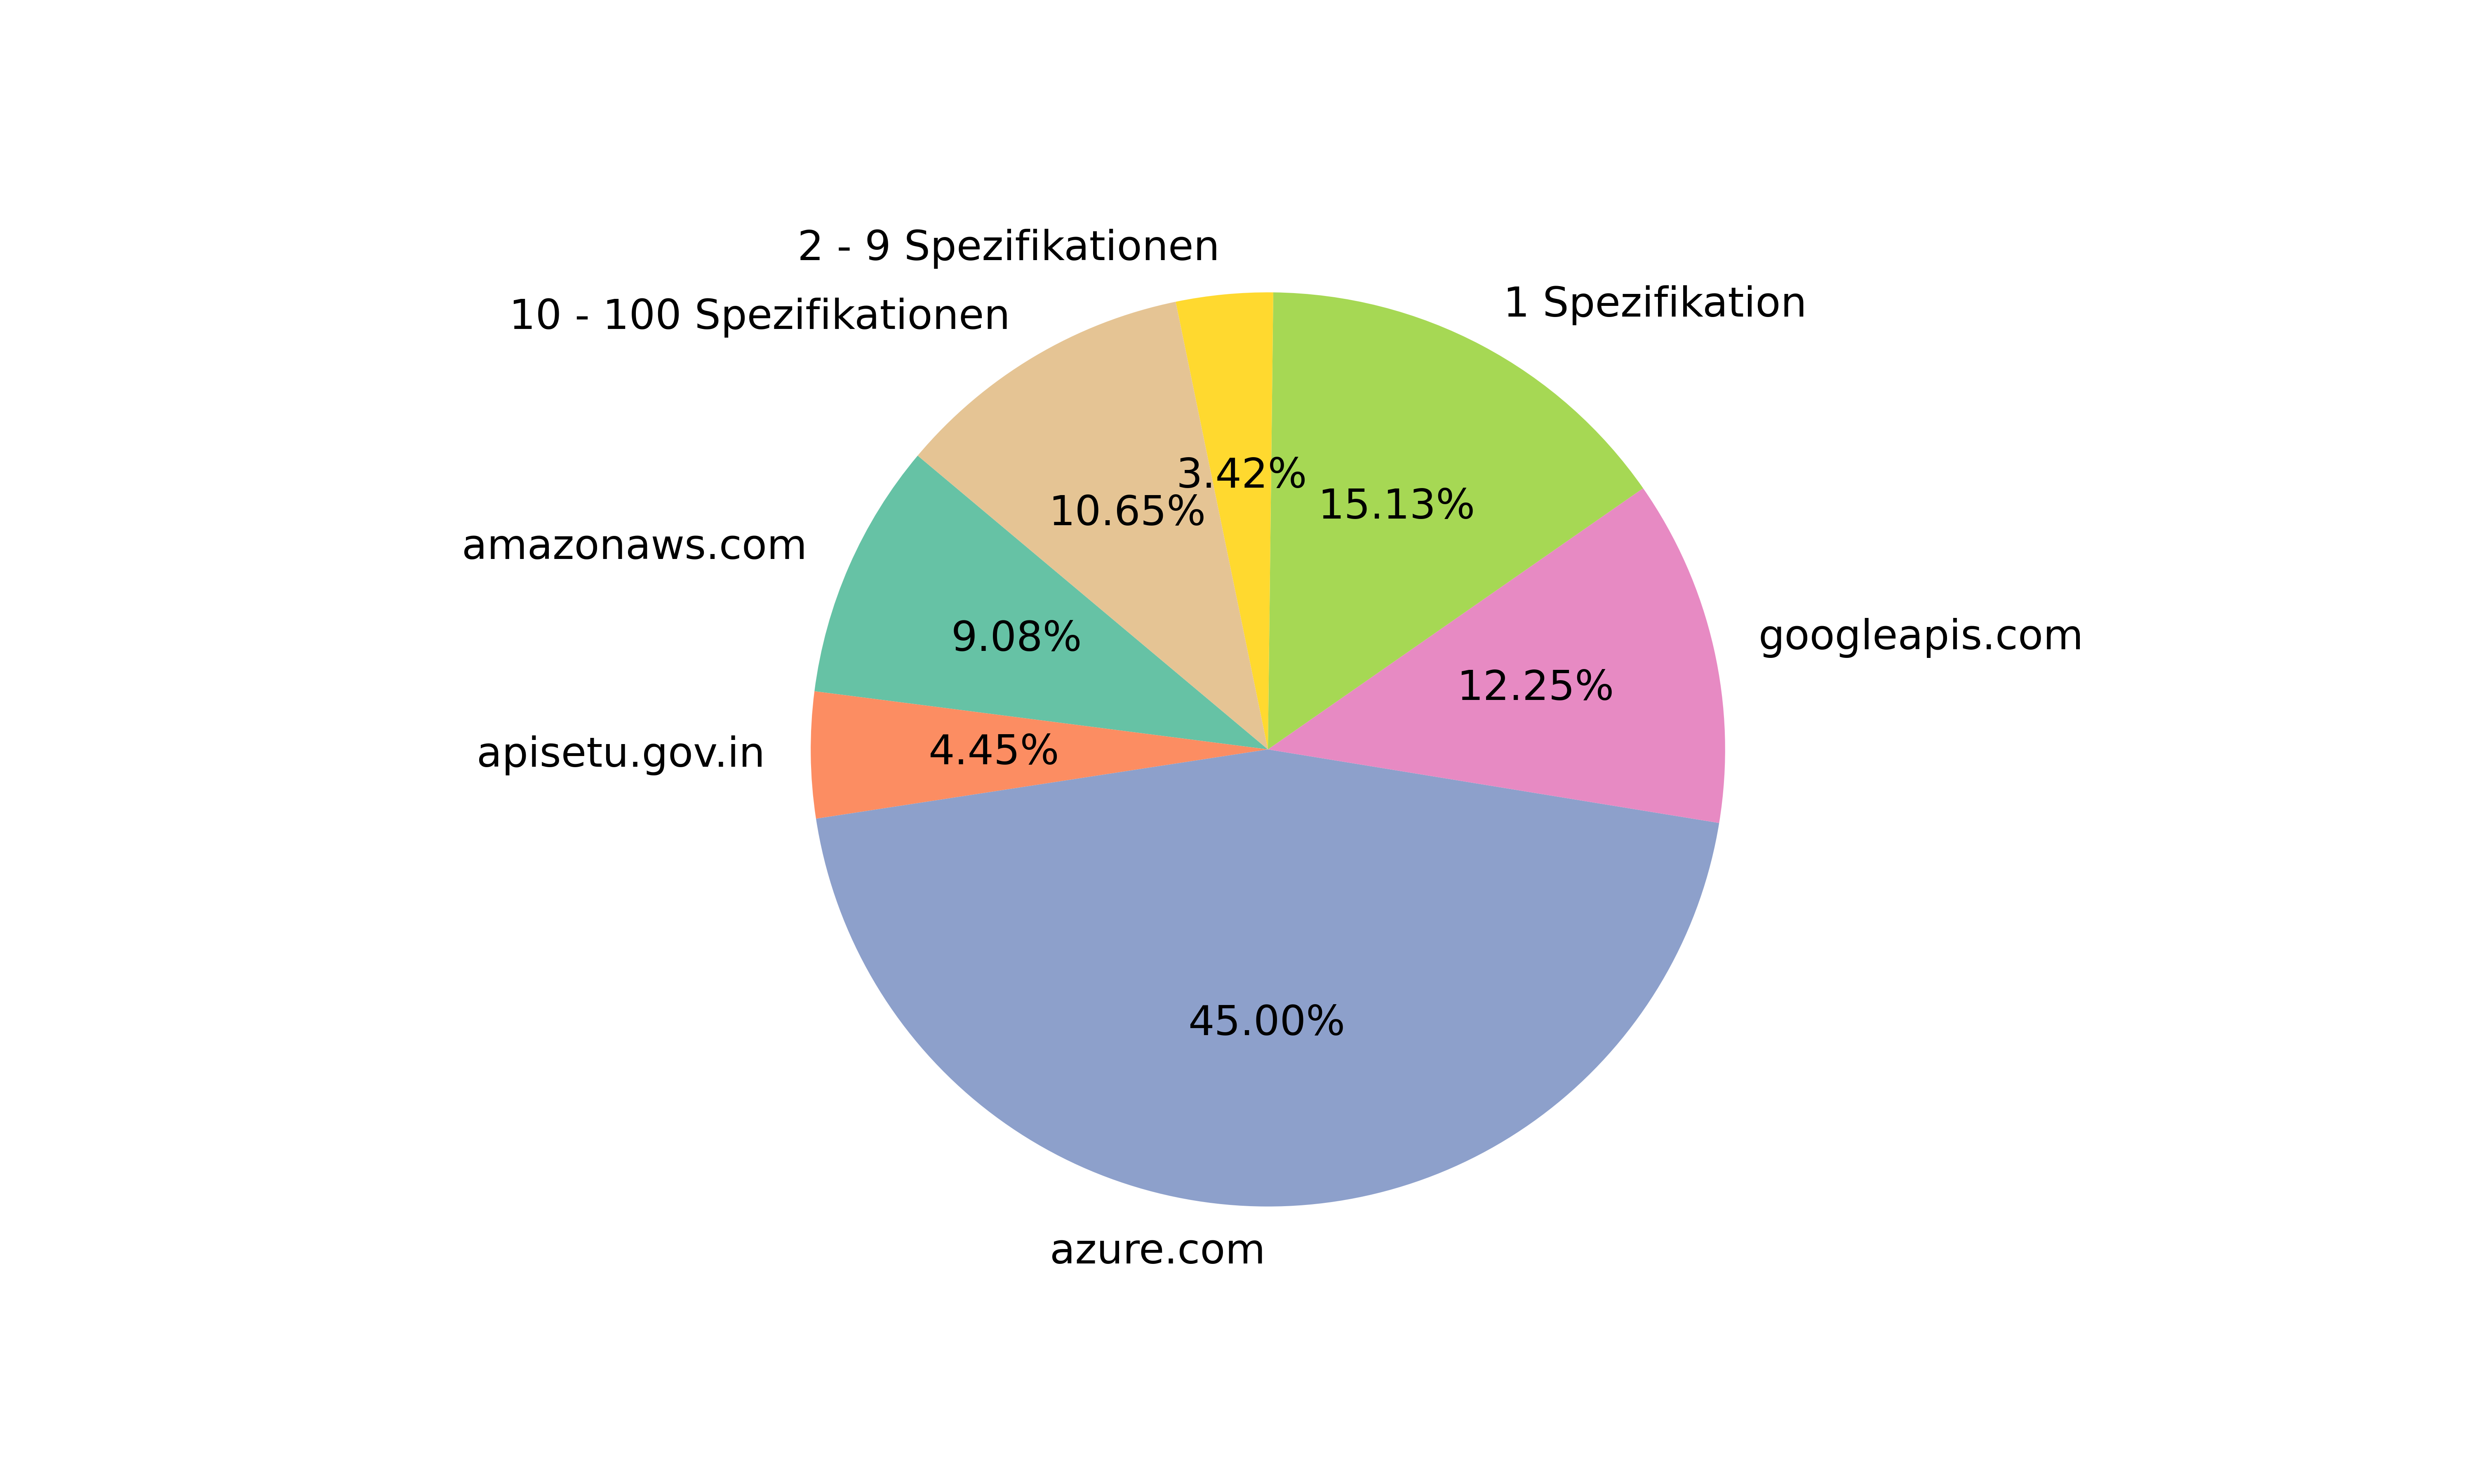
\includegraphics[width=0.9\linewidth]{img/specificationsperdomainpie.png}
  \caption{Anzahl der Spezifikationen pro Anbieter im OpenAPI Directory}
  \label{fig:Specifications}
\end{figure}

\newpage
Die Größe einer Spezifikation lässt sich durch die Anzahl der \acs{API} Operationen beschreiben. Die Größe einer OpenAPI Spezifikationen kann auch mit dem path Objekt gemessen werden \parencite{bogner_restruler_2024}. Jedes path Objekt enthält API Operationen für die darauf definierten \acs{HTTP} Methoden. 

Die tatsächliche Anzahl der Endpunkte einer OpenAPI Spezifikation entspricht daher einem multiplikativem Vielfachen der Anzahl der path Objekte. Daher werden in dieser Arbeit API Operationen als Kennzahl der Größe einer OpenAPI Spezifikation verwendet.
Spezifikationen im OpenAPI Directory variieren stark (siehe Abbildung \ref{fig:Operations}) in ihrer Größe. Die größte Spezifikation ist die microsoft.com/graph Spezifikation mit 11422 Operationen. Die kleinste ist die 1forge.com Spezifikation mit 2 Operationen.
\begin{figure}[htbp]
  \centering
  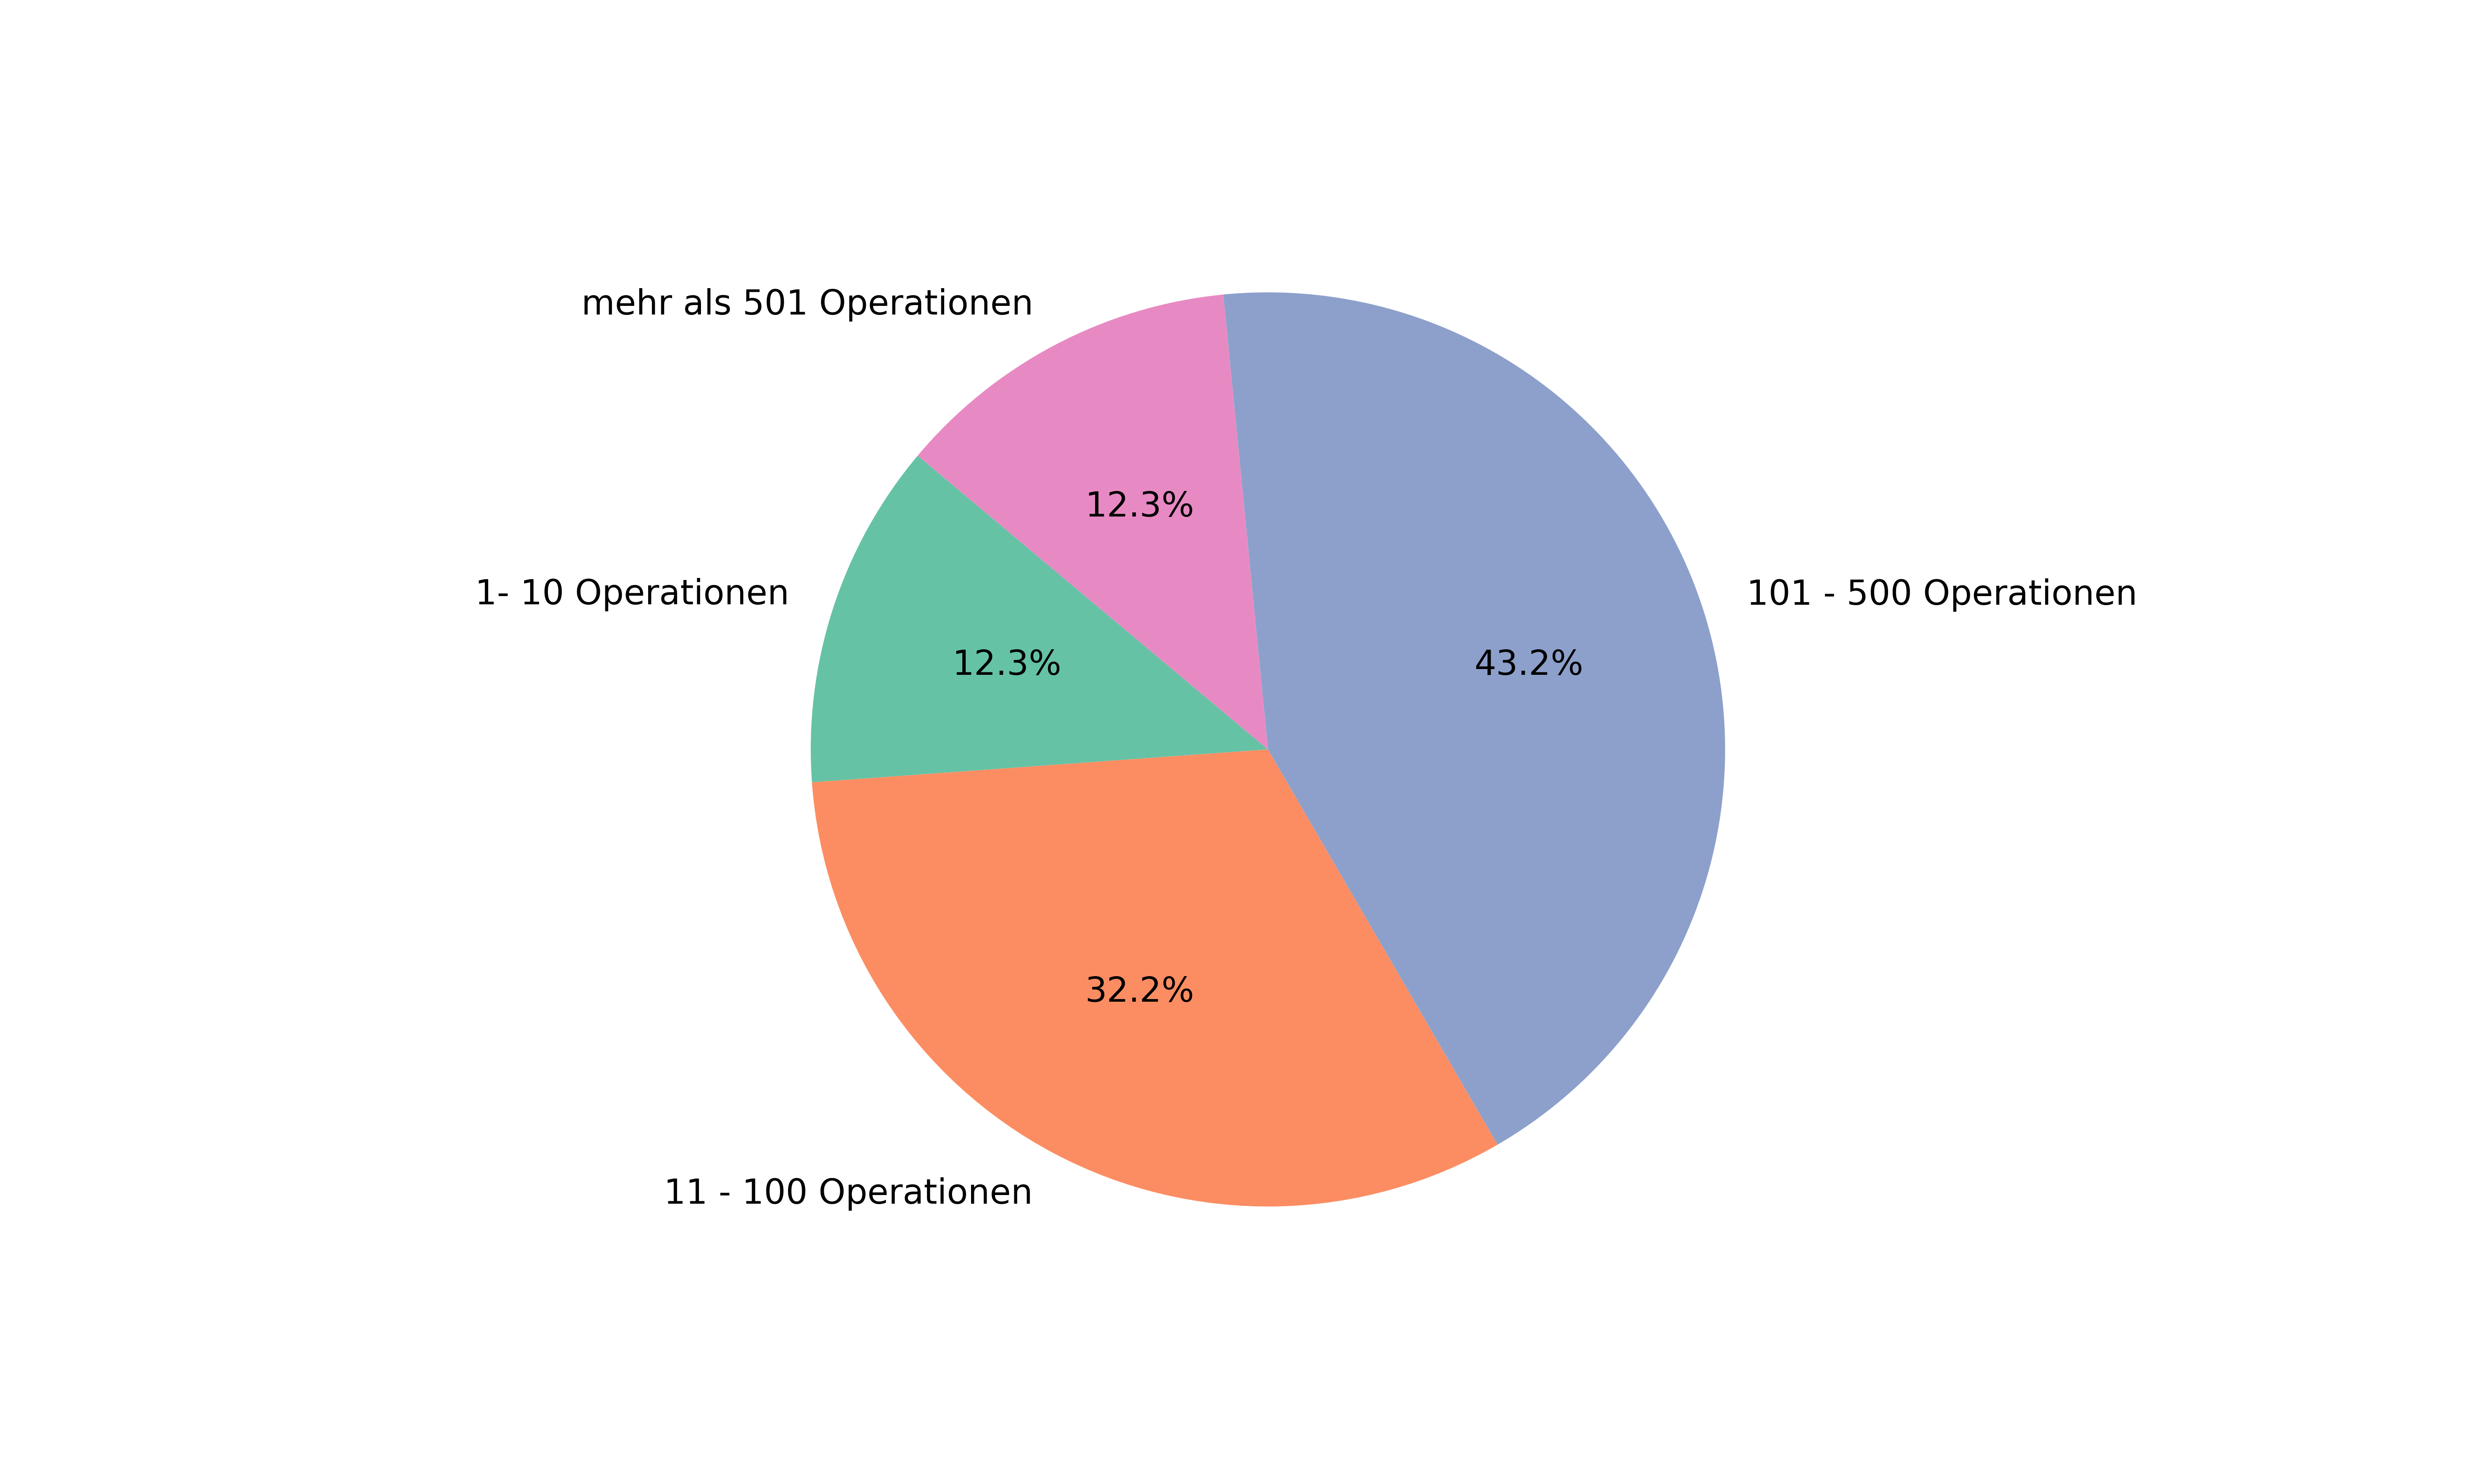
\includegraphics[width=0.9\linewidth]{img/operationsperspecificationpie.png}
  \caption{Anzahl der API Operationen pro Spezifikation im OpenAPI Directory}
  \label{fig:Operations}
\end{figure}

\subsection{Vergleichbare Studien} \label{sec:vergleichbarestudien}
Mehrere Arbeiten untersuchen bereits die genannten Themen, Konzepte, Technologien und Daten.
\parencite{palma_semantic_2017} entwickelt eine Methode um automatisiert linguistische Antipatterns in Web \acs{API}s zu detektieren. Diese Methode wird in \parencite{palma_specification_2014} mit dem Namen Service-Oriented Framework for Antipatterns (SOFA) implementiert.

In den drei Artikeln  \parencite{kotstein_which_2021}, \parencite{bogner_restful_2023} und \parencite{bogner_restruler_2024} untersucht Bogner systematisch die automatische Verifikation von \acs{REST} Qualitätsregeln nach \parencite{masse_rest_2011}. 

Zuerst werden \glqq Mismatches zwischen theoretischen \acs{REST} Konzepten und praktischen Implementierungen\grqq{} \parencite{kotstein_which_2021} identifiziert. Im Rahmen einer Delphi Studie \parencite{kotstein_which_2021} werden Industrieexperten mit einschlägiger Erfahrung zur Relevanz der Regeln aus \parencite{masse_rest_2011} befragt. Das Ergebnis des Delphi Konsensus ist, das nur ein kleiner Teil dieses Regelwerks in der Praxis als relevant empfunden wird. 

In der zweiten Studie \parencite{bogner_restful_2023} wird untersucht, ob Verstöße gegen die zuvor identifizierten wichtigen Regeln zu missverständlichen Interpretationen der Softwarespezifikation führen. Das Ergebnis ist, dass sowohl subjektives als auch objektives Verständnis einer Spezifikation mit Regelverstößen statistisch signifikant geringer ist, wenn die Regeln eingehalten werden. 

Die dritte Studie ist am ehesten vergleichbar mit dem Vorgehen dieser Arbeit. In dem Artikel wird ein Tool zur statischen Codeanalyse entworfen, das als Eingabe OpenAPI Spezifikationen akzeptiert und als Ausgabe Violations gegen selektierte \acs{REST}ful Prinzipien produziert. Als Grund für die Entwicklung eines eigenen Tools wird angegeben, das bestehende Tools (Spectral und Zally) sich ausschließlich auf Syntaxanalyse fokussieren und das Anlegen eines Regelwerks, das auf die Einhaltung von \acs{REST}ful Designprinzipien validiert deshalb nicht möglich sei \parencite{bogner_restruler_2024}\footnote{Diese Entscheidung ist angesichts der Mächtigkeit insbesondere von Spectral nicht ausreichend begründet. Spectral bietet über benutzerdefinierte JavaScript Funktionen die Möglichkeit innerhalb der Funktion auf den gesamten Kontext (OpenAPI Spezifikation und Regelwerk) zuzugreifen. Dies ermöglicht eine Analyse über syntaktische Kriterien hinaus.}. Im weiteren Verlauf wird ein Regelwerk mit 14 Regeln entwickelt, die in den vorhergehenden Studien als relevant identifiziert wurden. Im Verlauf der Studie werden die Regeln auf öffentlich verfügbare OpenAPI Spezifikationen aus dem APIs.guru Datensatz angewendet. Die Ergebnisse werden auf die Effektivität der Regeln und die Korrektheit des Tools untersucht. Das Ergebnis zeigt, dass sich \acs{REST}ful Designregeln gut an den OpenAPI Implementationen verifizieren lassen.

In \parencite{kim_leveraging_2024} wird ein \acf{LLM} verwendet, um \acs{REST}ful OpenAPI Spezifikationen zu interpretieren. Das Ziel ist es, anhand der Spezifikation und der enthaltenen Beschreibungen in natürlicher Sprache nützliche Beispiel \acs{API} Calls zu generieren. Es wird nur eine kleine Anzahl an praxisrelevanten OpenAPI Spezifikationen untersucht. Für zukünftige Studien plant \parencite{kim_leveraging_2024} auch das APIs.guru OpenAPI Directory zu verwenden. Der Fokus dieser Arbeit liegt auf dem funktionalen Testen der Schnittstellen, die die OpenAPI Spezifikationen beschreibt.

Zudem soll als Studie mit einem vergleichbaren Ansatz eine Bachelorarbeit genannt werden. In \parencite{eriksson_using_2023} wird ein Konzept vorgestellt, um die objektive Qualität von OpenAPI Spezifikationen zu bewerten. Dafür wird ein Spectral Regelwerk verwendet, dessen Regeln auf drei REST Qualitätsattribute abgebildet werden. Die generierten Linterfehler werden dann genutzt, um Googles  \acs{LLM} BERT zu trainieren und OpenAPI Spezifikationen einen objektiven Wert zuzuordnen.

Eine Studie zur empirischen Analyse von Linterregeln findet sich in \parencite{ferreira_campos_mining_2019}. Dort werden JavaScript Code Snippets der Online-Plattform Stack Overflow massenhaft mit dem JavaScript Linter ESLint untersucht. Die Studie kommt zu dem Schluss, dass alle dort veröffentlichten Snippets Linterfehler enthalten. Die meisten Linterfehler entsprachen der Kategorie stilistische Fehler. Mögliche logische Fehler im Code machten nur einen kleinen Anteil der Linterfehler aus. Eine anschließende Suche auf der Plattform GitHub konnte nachweisen, dass Snippets mit möglichen logischen Fehlern vielfältig in echten Projekten wiederverwendet wurden. 

Die genannten Studien zeigen, dass sich der OpenAPI Standard dazu eignet wissenschaftliche Studien zu aktuellen Softwareengineering Themen durchzuführen. Dass OpenAPI Spezifikationen aber nicht eindeutig sind und Qualitätsunterschiede zwischen verschiedenen Implementierungen vorliegen wurde zum jetzigen Stand nicht untersucht. Einige Regelwerke wurden bereits für solche Studien verwendet. Das Spectral \acs{OAS} Regelwerk, das das Standardregelwerk des populären Spectral \acs{API} Linters ist, wurde bisher nicht empirisch untersucht.
